
Este apêndice tem como objetivo registrar os dados obtidos durante a execução dos cenários de teste. Ao longo do apêndice, estão presentes
imagens do processo de auto-localização e do resultado da localização, como pode ser observado a seguir.


\section{Cenário de Teste 1}

Este cenário está dividido em 5 (cinco) exemplos, os quais são apresentados a seguir, contemplando todo o processo de auto-localização
em cada exemplo, a partir da apresentação das Imagens abaixo.

\subsection{Exemplo 1}

Exemplo utilizando 200 partículas:

\begin{figure}[H]
  \centering
  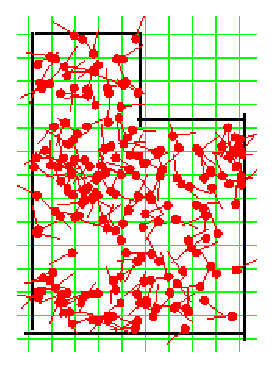
\includegraphics[scale=1]{figuras/cen1_ex1/1.eps}
  \caption[Partículas Iniciais]{Partículas iniciais}
  \label{img:cen1_ex1_1}
\end{figure}

\begin{figure}[H]
  \centering
  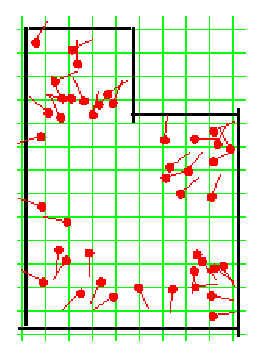
\includegraphics[scale=1]{figuras/cen1_ex1/2.eps}
  \caption[Primeiro Ciclo de Filtragem]{Primeiro ciclo de filtragem}
  \label{img:cen1_ex1_2}
\end{figure}

\begin{figure}[H]
  \centering
  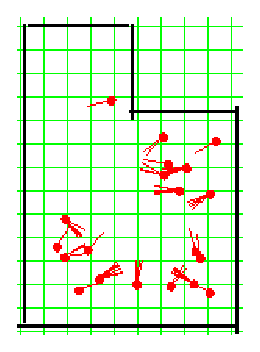
\includegraphics[scale=1]{figuras/cen1_ex1/3.eps}
  \caption[Segundo Ciclo de Filtragem]{Segundo ciclo de filtragem}
  \label{img:cen1_ex1_3}
\end{figure}

\begin{figure}[H]
  \centering
  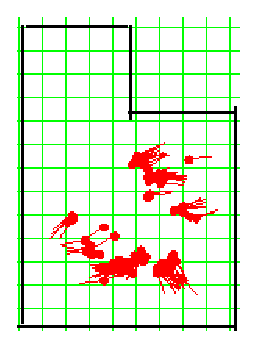
\includegraphics[scale=1]{figuras/cen1_ex1/4.eps}
  \caption[Terceiro Ciclo de Filtragem]{Terceiro ciclo de filtragem}
  \label{img:cen1_ex1_4}
\end{figure}

\begin{figure}[H]
  \centering
  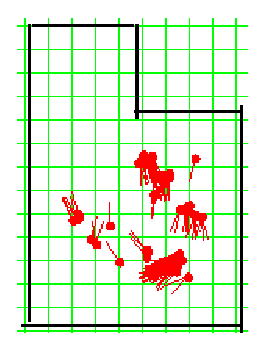
\includegraphics[scale=1]{figuras/cen1_ex1/5.eps}
  \caption[Quarto Ciclo de Filtragem]{Quarto ciclo de filtragem}
  \label{img:cen1_ex1_5}
\end{figure}

\begin{figure}[H]
  \centering
  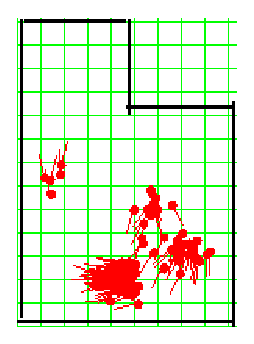
\includegraphics[scale=1]{figuras/cen1_ex1/6.eps}
  \caption[Quinto Ciclo de Filtragem]{Quinto ciclo de filtragem}
  \label{img:cen1_ex1_6}
\end{figure}

\begin{figure}[H]
  \centering
  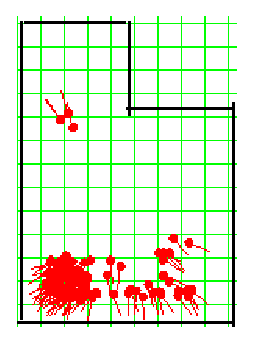
\includegraphics[scale=1]{figuras/cen1_ex1/7.eps}
  \caption[Sexto Ciclo de Filtragem]{Sexto ciclo de filtragem}
  \label{img:cen1_ex1_7}
\end{figure}

\begin{figure}[H]
  \centering
  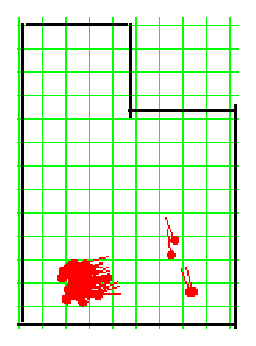
\includegraphics[scale=1]{figuras/cen1_ex1/8.eps}
  \caption[Sétimo Ciclo de Filtragem]{Sétimo ciclo de filtragem}
  \label{img:cen1_ex1_8}
\end{figure}

\begin{figure}[H]
  \centering
  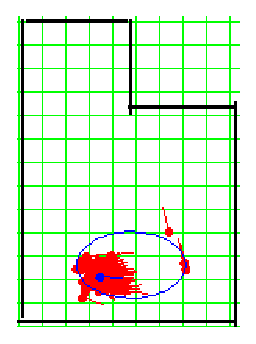
\includegraphics[scale=1]{figuras/cen1_ex1/9.eps}
  \caption[Oitavo Ciclo de Filtragem]{Oitavo ciclo de filtragem}
  \label{img:cen1_ex1_9}
\end{figure}

\begin{figure}[H]
  \centering
  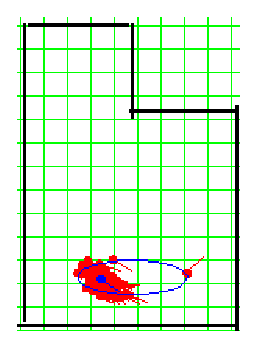
\includegraphics[scale=1]{figuras/cen1_ex1/10.eps}
  \caption[Nono Ciclo de Filtragem]{Nono ciclo de filtragem}
  \label{img:cen1_ex1_10}
\end{figure}

\subsection{Exemplo 2}

Exemplo utilizando 400 partículas:

\begin{figure}[H]
  \centering
  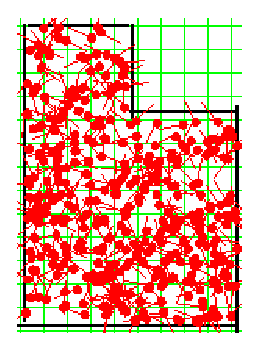
\includegraphics[scale=1]{figuras/cen1_ex2/1.eps}
  \caption[Partículas Iniciais]{Partículas iniciais}
  \label{img:cen1_ex2_1}
\end{figure}

\begin{figure}[H]
  \centering
  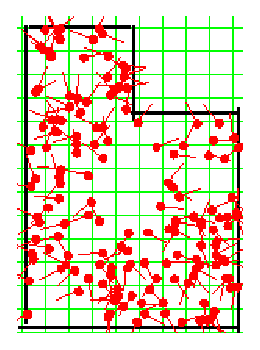
\includegraphics[scale=1]{figuras/cen1_ex2/2.eps}
  \caption[Primeiro Ciclo de Filtragem]{Primeiro ciclo de filtragem}
  \label{img:cen1_ex2_2}
\end{figure}

\begin{figure}[H]
  \centering
  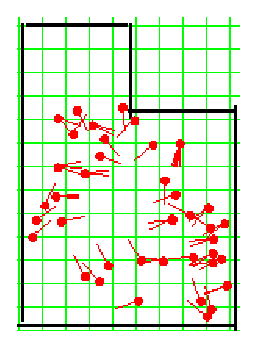
\includegraphics[scale=1]{figuras/cen1_ex2/3.eps}
  \caption[Segundo Ciclo de Filtragem]{Segundo ciclo de filtragem}
  \label{img:cen1_ex2_3}
\end{figure}

\begin{figure}[H]
  \centering
  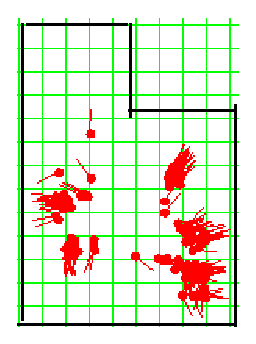
\includegraphics[scale=1]{figuras/cen1_ex2/4.eps}
  \caption[Terceiro Ciclo de Filtragem]{Terceiro ciclo de filtragem}
  \label{img:cen1_ex2_4}
\end{figure}

\begin{figure}[H]
  \centering
  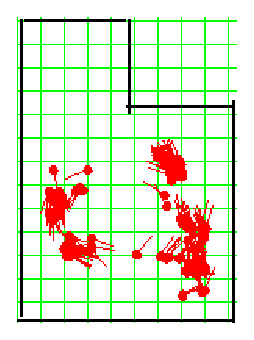
\includegraphics[scale=1]{figuras/cen1_ex2/5.eps}
  \caption[Quarto Ciclo de Filtragem]{Quarto ciclo de filtragem}
  \label{img:cen1_ex2_5}
\end{figure}

\begin{figure}[H]
  \centering
  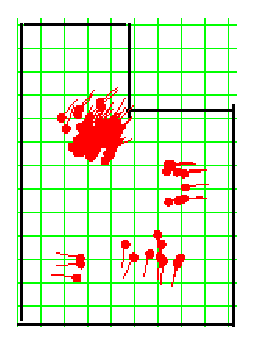
\includegraphics[scale=1]{figuras/cen1_ex2/6.eps}
  \caption[Quinto Ciclo de Filtragem]{Quinto ciclo de filtragem}
  \label{img:cen1_ex2_6}
\end{figure}

\begin{figure}[H]
  \centering
  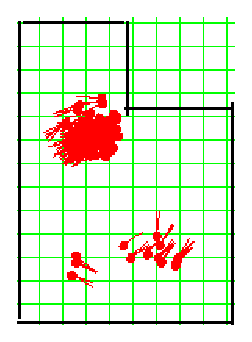
\includegraphics[scale=1]{figuras/cen1_ex2/7.eps}
  \caption[Sexto Ciclo de Filtragem]{Sexto ciclo de filtragem}
  \label{img:cen1_ex2_7}
\end{figure}

\begin{figure}[H]
  \centering
  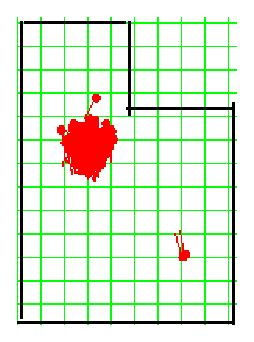
\includegraphics[scale=1]{figuras/cen1_ex2/8.eps}
  \caption[Sétimo Ciclo de Filtragem]{Sétimo ciclo de filtragem}
  \label{img:cen1_ex2_8}
\end{figure}

\begin{figure}[H]
  \centering
  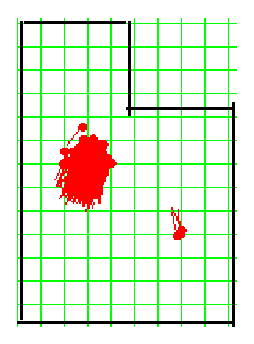
\includegraphics[scale=1]{figuras/cen1_ex2/9.eps}
  \caption[Oitavo Ciclo de Filtragem]{Oitavo ciclo de filtragem}
  \label{img:cen1_ex2_9}
\end{figure}

\begin{figure}[H]
  \centering
  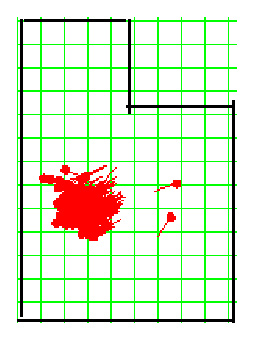
\includegraphics[scale=1]{figuras/cen1_ex2/10.eps}
  \caption[Nono Ciclo de Filtragem]{Nono ciclo de filtragem}
  \label{img:cen1_ex2_10}
\end{figure}

\begin{figure}[H]
  \centering
  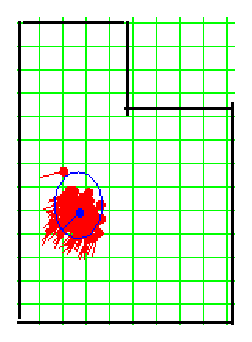
\includegraphics[scale=1]{figuras/cen1_ex2/11.eps}
  \caption[Décimo Ciclo de Filtragem]{Décimo ciclo de filtragem}
  \label{img:cen1_ex2_11}
\end{figure}

\subsection{Exemplo 3}

Exemplo utilizando 500 partículas:

\begin{figure}[H]
  \centering
  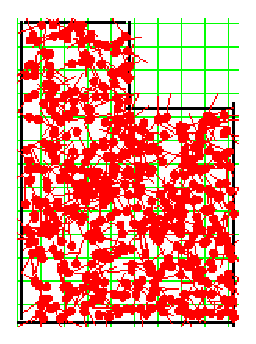
\includegraphics[scale=1]{figuras/cen1_ex3/1.eps}
  \caption[Partículas Iniciais]{Partículas iniciais}
  \label{img:cen1_ex3_1}
\end{figure}

\begin{figure}[H]
  \centering
  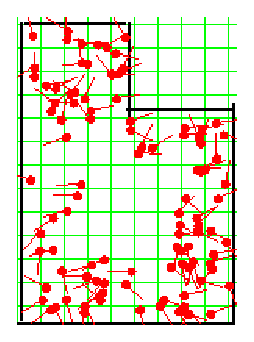
\includegraphics[scale=1]{figuras/cen1_ex3/2.eps}
  \caption[Primeiro Ciclo de Filtragem]{Primeiro ciclo de filtragem}
  \label{img:cen1_ex3_2}
\end{figure}

\begin{figure}[H]
  \centering
  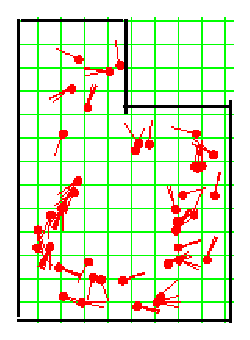
\includegraphics[scale=1]{figuras/cen1_ex3/3.eps}
  \caption[Segundo Ciclo de Filtragem]{Segundo ciclo de filtragem}
  \label{img:cen1_ex3_3}
\end{figure}

\begin{figure}[H]
  \centering
  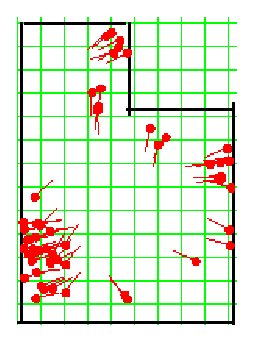
\includegraphics[scale=1]{figuras/cen1_ex3/4.eps}
  \caption[Terceiro Ciclo de Filtragem]{Terceiro ciclo de filtragem}
  \label{img:cen1_ex3_4}
\end{figure}

\begin{figure}[H]
  \centering
  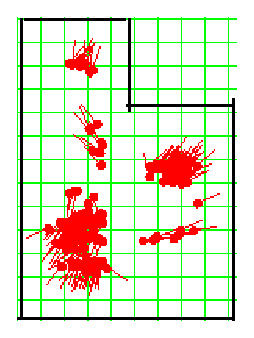
\includegraphics[scale=1]{figuras/cen1_ex3/5.eps}
  \caption[Quarto Ciclo de Filtragem]{Quarto ciclo de filtragem}
  \label{img:cen1_ex3_5}
\end{figure}

\begin{figure}[H]
  \centering
  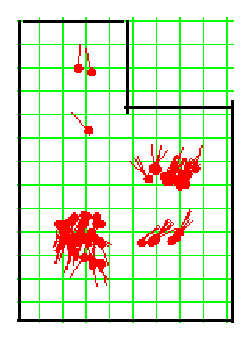
\includegraphics[scale=1]{figuras/cen1_ex3/6.eps}
  \caption[Quinto Ciclo de Filtragem]{Quinto ciclo de filtragem}
  \label{img:cen1_ex3_6}
\end{figure}

\begin{figure}[H]
  \centering
  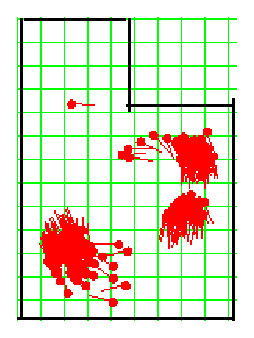
\includegraphics[scale=1]{figuras/cen1_ex3/7.eps}
  \caption[Sexto Ciclo de Filtragem]{Sexto ciclo de filtragem}
  \label{img:cen1_ex3_7}
\end{figure}

\begin{figure}[H]
  \centering
  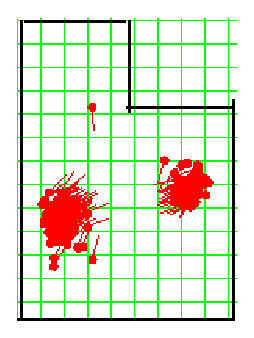
\includegraphics[scale=1]{figuras/cen1_ex3/8.eps}
  \caption[Sétimo Ciclo de Filtragem]{Sétimo ciclo de filtragem}
  \label{img:cen1_ex3_8}
\end{figure}

\begin{figure}[H]
  \centering
  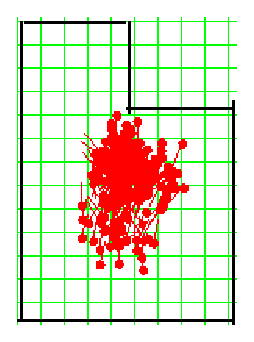
\includegraphics[scale=1]{figuras/cen1_ex3/9.eps}
  \caption[Oitavo Ciclo de Filtragem]{Oitavo ciclo de filtragem}
  \label{img:cen1_ex3_9}
\end{figure}

\begin{figure}[H]
  \centering
  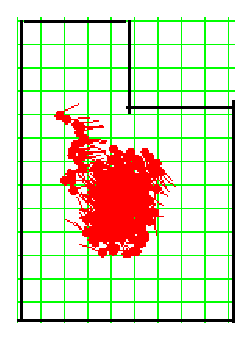
\includegraphics[scale=1]{figuras/cen1_ex3/10.eps}
  \caption[Nono Ciclo de Filtragem]{Nono ciclo de filtragem}
  \label{img:cen1_ex3_10}
\end{figure}

\begin{figure}[H]
  \centering
  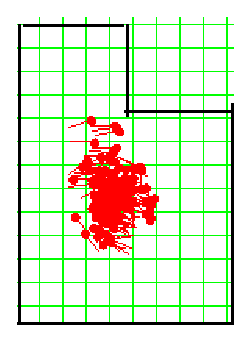
\includegraphics[scale=1]{figuras/cen1_ex3/11.eps}
  \caption[Décimo Ciclo de Filtragem]{Décimo ciclo de filtragem}
  \label{img:cen1_ex3_11}
\end{figure}

\begin{figure}[H]
  \centering
  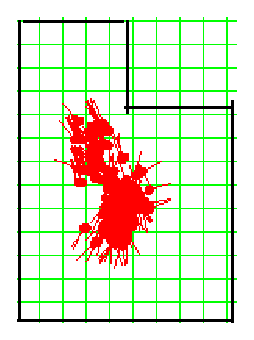
\includegraphics[scale=1]{figuras/cen1_ex3/12.eps}
  \caption[Décimo Primeiro Ciclo de Filtragem]{Décimo Primeiro ciclo de filtragem}
  \label{img:cen1_ex3_12}
\end{figure}

\begin{figure}[H]
  \centering
  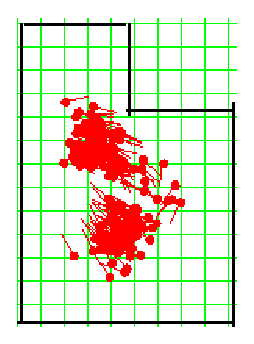
\includegraphics[scale=1]{figuras/cen1_ex3/13.eps}
  \caption[Décimo Segundo Ciclo de Filtragem]{Décimo Segundo ciclo de filtragem}
  \label{img:cen1_ex3_13}
\end{figure}

\begin{figure}[H]
  \centering
  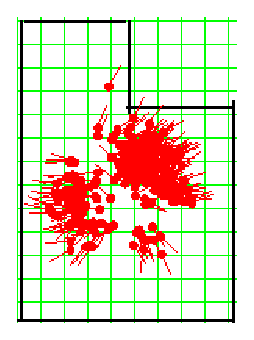
\includegraphics[scale=1]{figuras/cen1_ex3/14.eps}
  \caption[Décimo Terceiro Ciclo de Filtragem]{Décimo Terceiro ciclo de filtragem}
  \label{img:cen1_ex3_14}
\end{figure}

\begin{figure}[H]
  \centering
  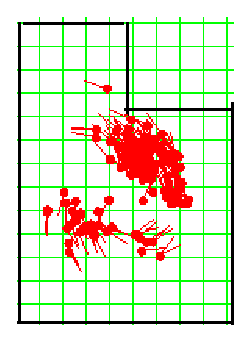
\includegraphics[scale=1]{figuras/cen1_ex3/15.eps}
  \caption[Décimo Quarto Ciclo de Filtragem]{Décimo Quarto ciclo de filtragem}
  \label{img:cen1_ex3_15}
\end{figure}

\begin{figure}[H]
  \centering
  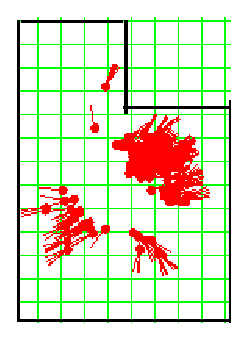
\includegraphics[scale=1]{figuras/cen1_ex3/16.eps}
  \caption[Décimo Quinto Ciclo de Filtragem]{Décimo Quinto ciclo de filtragem}
  \label{img:cen1_ex3_16}
\end{figure}

\begin{figure}[H]
  \centering
  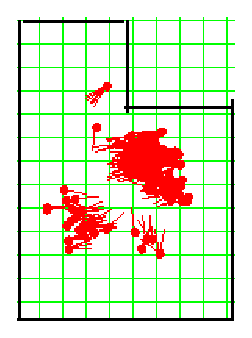
\includegraphics[scale=1]{figuras/cen1_ex3/17.eps}
  \caption[Décimo Sexto Ciclo de Filtragem]{Décimo Sexto ciclo de filtragem}
  \label{img:cen1_ex3_17}
\end{figure}

\begin{figure}[H]
  \centering
  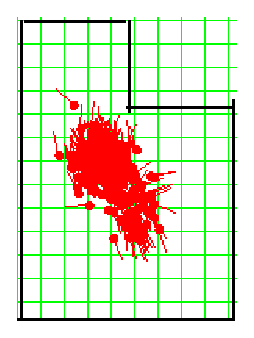
\includegraphics[scale=1]{figuras/cen1_ex3/18.eps}
  \caption[Décimo Sétimo Ciclo de Filtragem]{Décimo Sétimo ciclo de filtragem}
  \label{img:cen1_ex3_18}
\end{figure}

\begin{figure}[H]
  \centering
  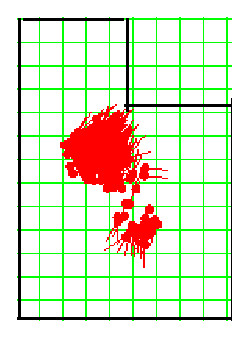
\includegraphics[scale=1]{figuras/cen1_ex3/19.eps}
  \caption[Décimo Oitavo Ciclo de Filtragem]{Décimo Oitavo ciclo de filtragem}
  \label{img:cen1_ex3_19}
\end{figure}

\begin{figure}[H]
  \centering
  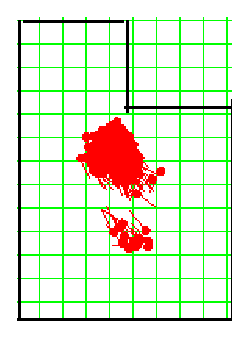
\includegraphics[scale=1]{figuras/cen1_ex3/20.eps}
  \caption[Décimo Nono Ciclo de Filtragem]{Décimo Nono ciclo de filtragem}
  \label{img:cen1_ex3_20}
\end{figure}

\begin{figure}[H]
  \centering
  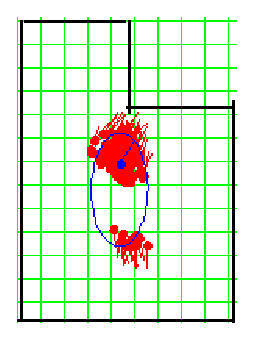
\includegraphics[scale=1]{figuras/cen1_ex3/21.eps}
  \caption[Vigésimo Ciclo de Filtragem]{Vigésimo ciclo de filtragem}
  \label{img:cen1_ex3_21}
\end{figure}

\begin{figure}[H]
  \centering
  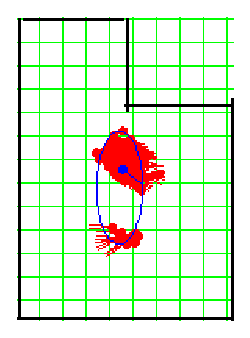
\includegraphics[scale=1]{figuras/cen1_ex3/22.eps}
  \caption[Vigésimo Primeiro Ciclo de Filtragem]{Vigésimo Primeiro ciclo de filtragem}
  \label{img:cen1_ex3_22}
\end{figure}

\begin{figure}[H]
  \centering
  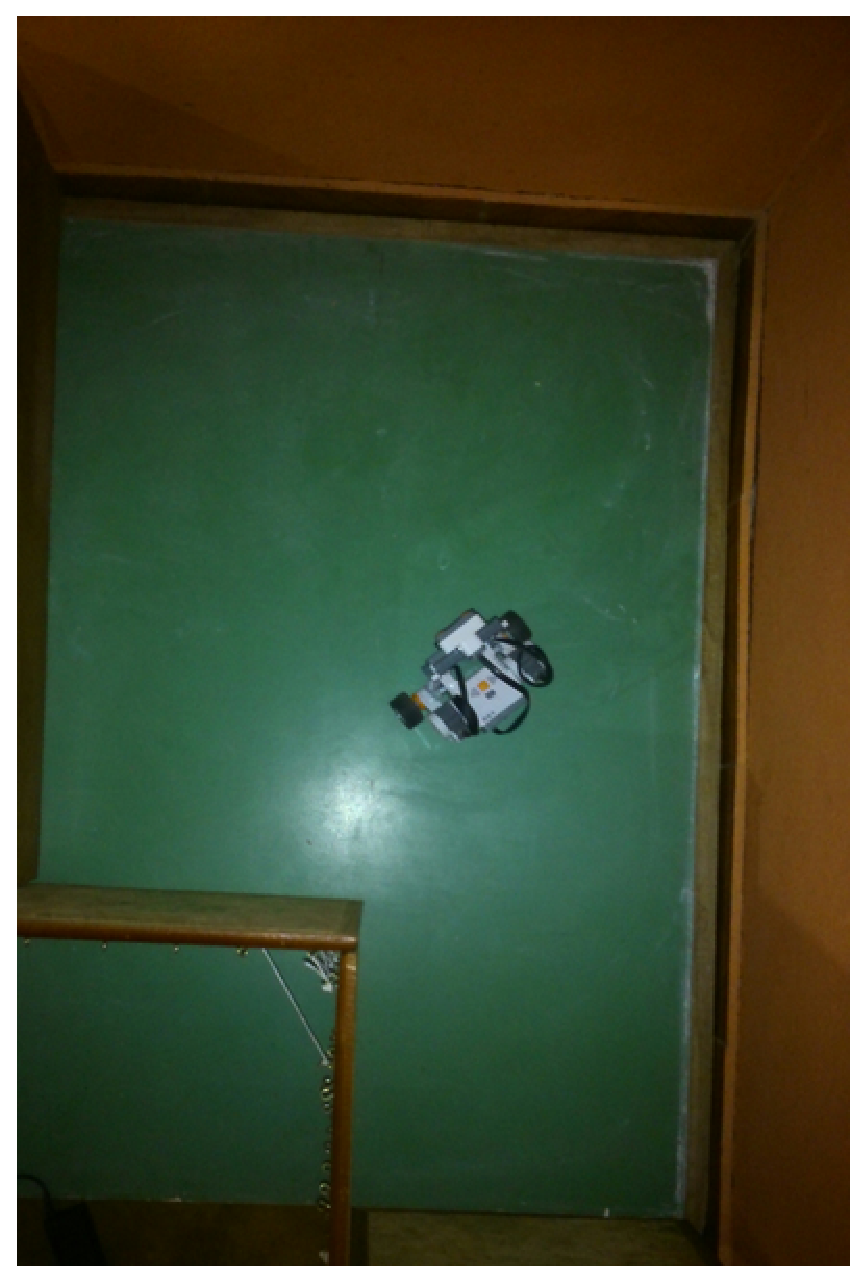
\includegraphics[scale=1]{figuras/cen1_ex3/real.eps}
  \caption[Posição Real do Robô]{Posição Real do Robô.}
  \label{img:cen1_ex3_23}
\end{figure}


\subsection{Exemplo 4}

Exemplo utilizando 100 partículas:

\begin{figure}[H]
  \centering
  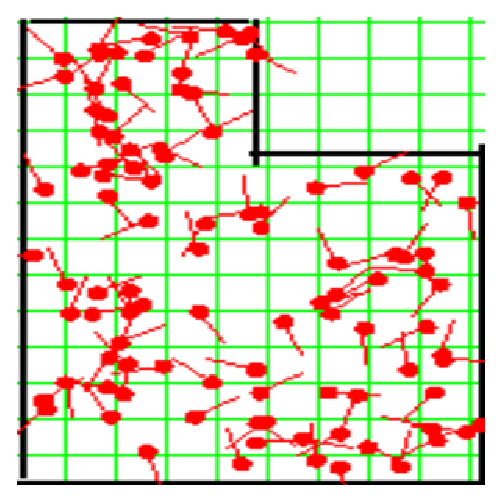
\includegraphics[scale=0.6]{figuras/cen1_ex4/1.eps}
  \caption[Partículas Iniciais]{Partículas iniciais}
  \label{img:cen1_ex4_1}
\end{figure}

\begin{figure}[H]
  \centering
  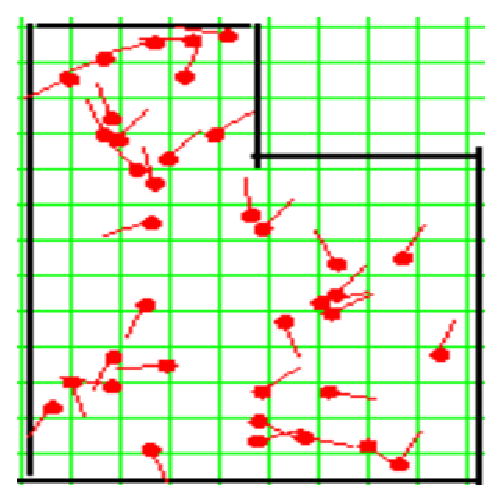
\includegraphics[scale=0.6]{figuras/cen1_ex4/2.eps}
  \caption[Primeiro Ciclo de Filtragem]{Primeiro ciclo de filtragem}
  \label{img:cen1_ex4_2}
\end{figure}

\begin{figure}[H]
  \centering
  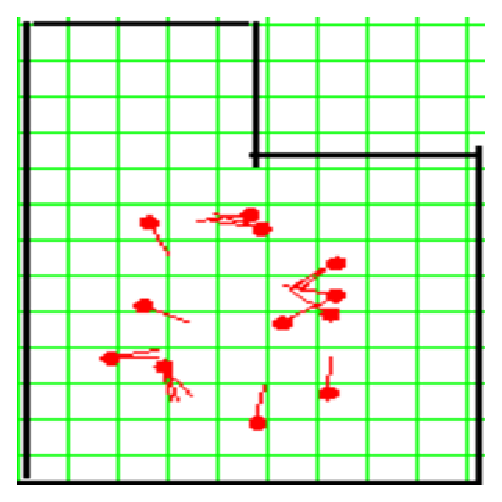
\includegraphics[scale=0.6]{figuras/cen1_ex4/3.eps}
  \caption[Segundo Ciclo de Filtragem]{Segundo ciclo de filtragem}
  \label{img:cen1_ex4_3}
\end{figure}

\begin{figure}[H]
  \centering
  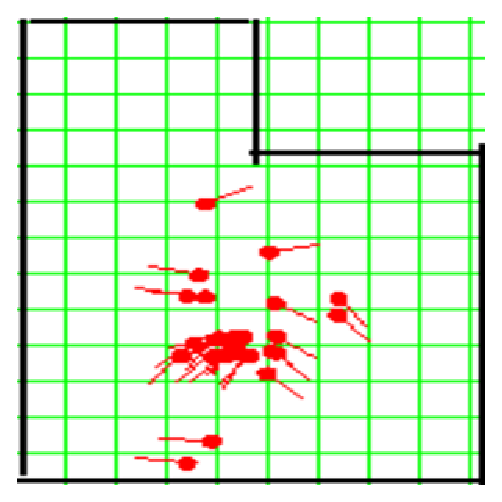
\includegraphics[scale=0.6]{figuras/cen1_ex4/4.eps}
  \caption[Terceiro Ciclo de Filtragem]{Terceiro ciclo de filtragem}
  \label{img:cen1_ex4_4}
\end{figure}

\begin{figure}[H]
  \centering
  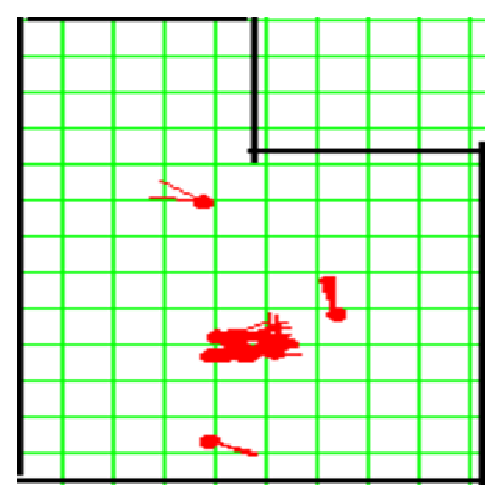
\includegraphics[scale=0.6]{figuras/cen1_ex4/5.eps}
  \caption[Quarto Ciclo de Filtragem]{Quarto ciclo de filtragem}
  \label{img:cen1_ex4_5}
\end{figure}

\begin{figure}[H]
  \centering
  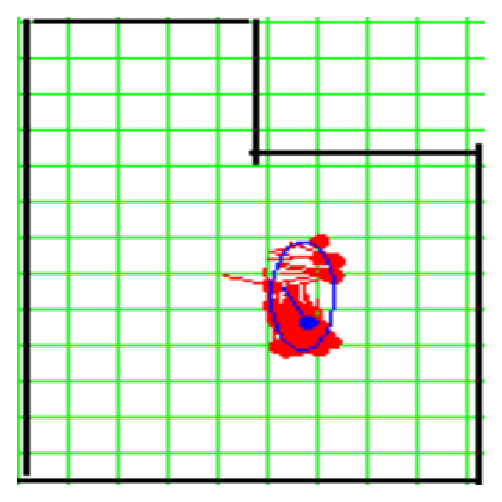
\includegraphics[scale=0.6]{figuras/cen1_ex4/6.eps}
  \caption[Quinto Ciclo de Filtragem]{Quinto ciclo de filtragem}
  \label{img:cen1_ex4_6}
\end{figure}

\begin{figure}[H]
  \centering
  \includegraphics[scale=0.8]{figuras/cen1_ex4/real.eps}
  \caption[Posição real do Robô]{Posição Real do Robô.}
  \label{img:cen1_ex4_6}
\end{figure}

\subsection{Exemplo 5}

Exemplo utilizando 150 partículas:

\begin{figure}[H]
  \centering
  \includegraphics[scale=1]{figuras/cen1_ex5/1.eps}
  \caption[Partículas Iniciais]{Partículas iniciais}
  \label{img:cen1_ex5_1}
\end{figure}

\begin{figure}[H]
  \centering
  \includegraphics[scale=1]{figuras/cen1_ex5/2.eps}
  \caption[Primeiro Ciclo de Filtragem]{Primeiro ciclo de filtragem}
  \label{img:cen1_ex5_2}
\end{figure}

\begin{figure}[H]
  \centering
  \includegraphics[scale=1]{figuras/cen1_ex5/3.eps}
  \caption[Segundo Ciclo de Filtragem]{Segundo ciclo de filtragem}
  \label{img:cen1_ex5_3}
\end{figure}

\begin{figure}[H]
  \centering
  \includegraphics[scale=1]{figuras/cen1_ex5/4.eps}
  \caption[Terceiro Ciclo de Filtragem]{Terceiro ciclo de filtragem}
  \label{img:cen1_ex5_4}
\end{figure}

\begin{figure}[H]
  \centering
  \includegraphics[scale=0.8]{figuras/cen1_ex5/real.eps}
  \caption[Posição real do Robô]{Posição Real do Robô.}
  \label{img:cen1_ex5_6}
\end{figure}

\section{Cenário de Teste 2}

Este cenário está dividido em 5 (cinco) exemplos, os quais são apresentados a seguir, contemplando todo o processo de auto-localização
em cada exemplo, a partir da apresentação das Imagens abaixo.

\subsection{Exemplo 1}

Exemplo utilizando velocidade de rotação em 10 graus por segundo:

\begin{figure}[H]
  \centering
  \includegraphics[scale=0.4]{figuras/cen2_ex1.eps}
  \caption[Cenário 2 - Exemplo 1]{Cenário 2 - Exemplo 1}
  \label{img:cen2_ex1}
\end{figure}

\subsection{Exemplo 2}

Exemplo utilizando velocidade de rotação em 30 graus por segundo:

\begin{figure}[H]
  \centering
  \includegraphics[scale=0.4]{figuras/cen2_ex2.eps}
  \caption[Cenário 2 - Exemplo 2]{Cenário 2 - Exemplo 2}
  \label{img:cen2_ex2}
\end{figure}

\subsection{Exemplo 3}

Exemplo utilizando velocidade de rotação em 50 graus por segundo:

\begin{figure}[H]
  \centering
  \includegraphics[scale=0.4]{figuras/cen2_ex3.eps}
  \caption[Cenário 2 - Exemplo 3]{Cenário 2 - Exemplo 3}
  \label{img:cen2_ex3}
\end{figure}

\subsection{Exemplo 4}

Exemplo utilizando velocidade de rotação em 70 graus por segundo:

\begin{figure}[H]
  \centering
  \includegraphics[scale=0.4]{figuras/cen2_ex4.eps}
  \caption[Cenário 2 - Exemplo 4]{Cenário 2 - Exemplo 4}
  \label{img:cen2_ex4}
\end{figure}

\subsection{Exemplo 5}

Exemplo utilizando velocidade de rotação em 90 graus por segundo:

\begin{figure}[H]
  \centering
  \includegraphics[scale=0.4]{figuras/cen2_ex5.eps}
  \caption[Cenário 2 - Exemplo 5]{Cenário 2 - Exemplo 5}
  \label{img:cen2_ex5}
\end{figure}

\section{Cenário de Teste 3}

Este cenário está dividido em 5 (cinco) exemplos, os quais são apresentados a seguir, contemplando todo o processo de auto-localização
em cada exemplo, a partir da apresentação das imagens a seguir, Figura \ref{img:cen3_ex1} a Figura \ref{img:real_cen3_ex5}.

\subsection{Exemplo 1}

Exemplo utilizando velocidade de deslocamento em 2 unidades de diâmetro por segundo:

{\centering
\includegraphics[scale=0.4]{figuras/cen3_ex1.eps}
\captionof{figure}{Cenário 3 - Exemplo 1}
\label{img:cen3_ex1}
\par}

{\centering
\includegraphics[scale=0.2]{figuras/real_cen3_ex1.eps}
\captionof{figure}{Posição Real do Cenário 3 - Exemplo 1.}
\label{img:real_cen3_ex1}
\par}


\subsection{Exemplo 2}

Exemplo utilizando velocidade de deslocamento em 5 unidades de diâmetro por segundo:

{\centering
\includegraphics[scale=0.4]{figuras/cen3_ex2.eps}
\captionof{figure}{Cenário 3 - Exemplo 2}
\label{img:cen3_ex2}
\par}

{\centering
\includegraphics[scale=0.2]{figuras/real_cen3_ex2.eps}
\captionof{figure}{Posição Real do Cenário 3 - Exemplo 2.}
\label{img:real_cen3_ex2}
\par}


\subsection{Exemplo 3}

Exemplo utilizando velocidade de deslocamento em 10 unidades de diâmetro por segundo:

{\centering
\includegraphics[scale=0.4]{figuras/cen3_ex3.eps}
\captionof{figure}{Cenário 3 - Exemplo 3}
\label{img:cen3_ex3}
\par}

{\centering
\includegraphics[scale=0.2]{figuras/real_cen3_ex3.eps}
\captionof{figure}{Posição Real do Cenário 3 - Exemplo 3.}
\label{img:real_cen3_ex3}
\par}

\subsection{Exemplo 4}

Exemplo utilizando velocidade de deslocamento em 15 unidades de diâmetro por segundo:

{\centering
\includegraphics[scale=0.4]{figuras/cen3_ex4.eps}
\captionof{figure}{Cenário 3 - Exemplo 4}
\label{img:cen3_ex4}
\par}

{\centering
\includegraphics[scale=0.2]{figuras/real_cen3_ex4.eps}
\captionof{figure}{Posição Real do Cenário 3 - Exemplo 4.}
\label{img:real_cen3_ex4}
\par}

\subsection{Exemplo 5}

Exemplo utilizando velocidade de deslocamento em 30 unidades de diâmetro por segundo:

{\centering
\includegraphics[scale=0.4]{figuras/cen3_ex5.eps}
\captionof{figure}{Cenário 3 - Exemplo 5}
\label{img:cen3_ex5}
\par}

{\centering
\includegraphics[scale=0.2]{figuras/real_cen3_ex5.eps}
\captionof{figure}{Posição Real do Cenário 3 - Exemplo 5.}
\label{img:real_cen3_ex5}
\par}

\section{Cenário de Teste 4}

Este cenário está dividido em 5 (cinco) exemplos, os quais são apresentados a seguir, contemplando todo o processo de auto-localização
em cada exemplo, a partir da apresentação das Imagens abaixo.

\subsection{Exemplo 1}

{\centering
\includegraphics[scale=0.4]{figuras/cen4_ex1.eps}
\captionof{figure}{Cenário 4 - Exemplo 1}
\label{img:cen4_ex1}
\par}

\subsection{Exemplo 2}

{\centering
\includegraphics[scale=0.4]{figuras/cen4_ex2.eps}
\captionof{figure}{Cenário 4 - Exemplo 2}
\label{img:cen4_ex2}
\par}

\subsection{Exemplo 3}

{\centering
\includegraphics[scale=0.4]{figuras/cen4_ex3.eps}
\captionof{figure}{Cenário 4 - Exemplo 3}
\label{img:cen4_ex3}
\par}

\subsection{Exemplo 4}

{\centering
\includegraphics[scale=0.4]{figuras/cen4_ex4.eps}
\captionof{figure}{Cenário 4 - Exemplo 4}
\label{img:cen4_ex4}
\par}

\subsection{Exemplo 5}

{\centering
\includegraphics[scale=0.4]{figuras/cen4_ex5.eps}
\captionof{figure}{Cenário 4 - Exemplo 5}
\label{img:cen4_ex5}
\par}

\section{Caso de Teste 5}
\label{sec:cenario5}

Este caso de teste está dividido em 5 (cinco) cenários, os quais são apresentados a seguir, contemplando todo o processo de auto-localização
em cada exemplo, a partir da apresentação das imagens a seguir, Figura \ref{img:cen5_ex1} a Figura \ref{img:real_cen5_ex5}.

\subsection{Cenário 1}

{\centering
\includegraphics[scale=0.4]{figuras/cen5_ex1.eps}
\captionof{figure}{Caso de Teste 5 - Cenário 1.}
\label{img:cen5_ex1}
\par}

{\centering
\includegraphics[scale=0.2]{figuras/real_cen5_ex1.eps}
\captionof{figure}{Posição Real do Caso de Teste 5 - Cenário 1.}
\label{img:real_cen5_ex1}
\par}

\subsection{Cenário 2}

{\centering
\includegraphics[scale=0.4]{figuras/cen5_ex2.eps}
\captionof{figure}{Caso de Teste 5 - Cenário 2.}
\label{img:cen5_ex2}
\par}

{\centering
\includegraphics[scale=0.2]{figuras/real_cen5_ex2.eps}
\captionof{figure}{Posição Real do Caso de Teste 5 - Cenário 2.}
\label{img:real_cen5_ex2}
\par}

\subsection{Cenário 3}

{\centering
\includegraphics[scale=0.4]{figuras/cen5_ex3.eps}
\captionof{figure}{Caso de Teste 5 - Cenário 3.}
\label{img:cen5_ex3}
\par}

{\centering
\includegraphics[scale=0.2]{figuras/real_cen5_ex3.eps}
\captionof{figure}{Posição Real do Caso de Teste 5 - Cenário 3.}
\label{img:real_cen5_ex3}
\par}

\subsection{Cenário 4}

{\centering
\includegraphics[scale=0.4]{figuras/cen5_ex4.eps}
\captionof{figure}{Caso de Teste 5 - Cenário 4.}
\label{img:cen5_ex4}
\par}

{\centering
\includegraphics[scale=0.2]{figuras/real_cen5_ex4.eps}
\captionof{figure}{Posição Real do Caso de Teste 5 - Cenário 4.}
\label{img:real_cen5_ex4}
\par}

\subsection{Cenário 5}

{\centering
\includegraphics[scale=0.4]{figuras/cen5_ex5.eps}
\captionof{figure}{Caso de Teste 5 - Cenário 5.}
\label{img:cen5_ex5}
\par}

{\centering
\includegraphics[scale=0.2]{figuras/real_cen5_ex5.eps}
\captionof{figure}{Posição Real do Caso de Teste 5 - Cenário 5.}
\label{img:real_cen5_ex5}
\par}

\section{Cenário de Teste 6}
\label{sec:cenario6}

Este cenário está dividido em 5 (cinco) exemplos, os quais são apresentados a seguir, contemplando todo o processo de auto-localização
em cada exemplo, a partir da apresentação das imagens a seguir, Figura \ref{img:cen6_ex1} a Figura \ref{img:real_cen6_ex5}.

\subsection{Exemplo 1}

{\centering
\includegraphics[scale=0.4]{figuras/cen6_ex1.eps}
\captionof{figure}{Cenário 6 - Exemplo 1.}
\label{img:cen6_ex1}
\par}

{\centering
\includegraphics[scale=0.2]{figuras/real_cen6_ex1.eps}
\captionof{figure}{Posição Real do Cenário 6 - Exemplo 1.}
\label{img:real_cen6_ex1}
\par}

\subsection{Exemplo 2}

{\centering
\includegraphics[scale=0.4]{figuras/cen6_ex2.eps}
\captionof{figure}{Cenário 6 - Exemplo 2.}
\label{img:cen6_ex2}
\par}

{\centering
\includegraphics[scale=0.2]{figuras/real_cen6_ex2.eps}
\captionof{figure}{Posição Real do Cenário 6 - Exemplo 2.}
\label{img:real_cen6_ex2}
\par}

\subsection{Exemplo 3}

{\centering
\includegraphics[scale=0.4]{figuras/cen6_ex3.eps}
\captionof{figure}{Cenário 6 - Exemplo 3.}
\label{img:cen6_ex3}
\par}

{\centering
\includegraphics[scale=0.2]{figuras/real_cen6_ex3.eps}
\captionof{figure}{Posição Real do Cenário 6 - Exemplo 3.}
\label{img:real_cen6_ex3}
\par}

\subsection{Exemplo 4}

{\centering
\includegraphics[scale=0.4]{figuras/cen6_ex4.eps}
\captionof{figure}{Cenário 6 - Exemplo 4.}
\label{img:cen6_ex4}
\par}

{\centering
\includegraphics[scale=0.2]{figuras/real_cen6_ex4.eps}
\captionof{figure}{Posição Real do Cenário 6 - Exemplo 4.}
\label{img:real_cen6_ex4}
\par}

\subsection{Exemplo 5}

{\centering
\includegraphics[scale=0.4]{figuras/cen6_ex5.eps}
\captionof{figure}{Cenário 6 - Exemplo 5.}
\label{img:cen6_ex5}
\par}

{\centering
\includegraphics[scale=0.2]{figuras/real_cen6_ex5.eps}
\captionof{figure}{Posição Real do Cenário 6 - Exemplo 5.}
\label{img:real_cen6_ex5}
\par}

\section{Cenário de Teste 7}
\label{sec:cenario7}

Este cenário está dividido em 5 (cinco) exemplos, os quais são apresentados a seguir, contemplando todo o processo de auto-localização
em cada exemplo, a partir da apresentação das imagens a seguir, Figura \ref{img:cen7_ex1} a Figura \ref{img:real_cen7_ex5}.

\subsection{Exemplo 1}

{\centering
\includegraphics[scale=0.4]{figuras/cen7_ex1.eps}
\captionof{figure}{Cenário 7 - Exemplo 1.}
\label{img:cen7_ex1}
\par}

{\centering
\includegraphics[scale=0.2]{figuras/real_cen7_ex1.eps}
\captionof{figure}{Posição Real do Cenário 7 - Exemplo 1.}
\label{img:real_cen7_ex1}
\par}

\subsection{Exemplo 2}

{\centering
\includegraphics[scale=0.4]{figuras/cen7_ex2.eps}
\captionof{figure}{Cenário 7 - Exemplo 2.}
\label{img:cen7_ex2}
\par}

{\centering
\includegraphics[scale=0.2]{figuras/real_cen7_ex2.eps}
\captionof{figure}{Posição Real do Cenário 7 - Exemplo 2.}
\label{img:real_cen7_ex2}
\par}

\subsection{Exemplo 3}

{\centering
\includegraphics[scale=0.4]{figuras/cen7_ex3.eps}
\captionof{figure}{Cenário 7 - Exemplo 3.}
\label{img:cen7_ex3}
\par}

{\centering
\includegraphics[scale=0.2]{figuras/real_cen7_ex3.eps}
\captionof{figure}{Posição Real do Cenário 7 - Exemplo 3.}
\label{img:real_cen7_ex3}
\par}

\subsection{Exemplo 4}

{\centering
\includegraphics[scale=0.4]{figuras/cen7_ex4.eps}
\captionof{figure}{Cenário 7 - Exemplo 4.}
\label{img:cen7_ex4}
\par}

{\centering
\includegraphics[scale=0.2]{figuras/real_cen7_ex4.eps}
\captionof{figure}{Posição Real do Cenário 7 - Exemplo 4.}
\label{img:real_cen7_ex4}
\par}

\subsection{Exemplo 5}

{\centering
\includegraphics[scale=0.4]{figuras/cen7_ex5.eps}
\captionof{figure}{Cenário 7 - Exemplo 5.}
\label{img:cen7_ex5}
\par}

{\centering
\includegraphics[scale=0.2]{figuras/real_cen7_ex5.eps}
\captionof{figure}{Posição Real do Cenário 7 - Exemplo 5.}
\label{img:real_cen7_ex5}
\par}

\section{Cenário de Teste 8}
\label{sec:cenario8}

Este cenário está dividido em 5 (cinco) exemplos, os quais são apresentados a seguir, contemplando todo o processo de auto-localização
em cada exemplo, a partir da apresentação das imagens a seguir, Figura \ref{img:cen8_ex1} a Figura \ref{img:real_cen8_ex5}.

\subsection{Exemplo 1}

{\centering
\includegraphics[scale=0.4]{figuras/cen8_ex1.eps}
\captionof{figure}{Cenário 8 - Exemplo 1.}
\label{img:cen8_ex1}
\par}

{\centering
\includegraphics[scale=0.2]{figuras/real_cen8_ex1.eps}
\captionof{figure}{Posição Real do Cenário 8 - Exemplo 1.}
\label{img:real_cen8_ex1}
\par}

\subsection{Exemplo 2}

{\centering
\includegraphics[scale=0.4]{figuras/cen8_ex2.eps}
\captionof{figure}{Cenário 8 - Exemplo 2.}
\label{img:cen8_ex2}
\par}

{\centering
\includegraphics[scale=0.2]{figuras/real_cen8_ex2.eps}
\captionof{figure}{Posição Real do Cenário 8 - Exemplo 2.}
\label{img:real_cen8_ex2}
\par}

\subsection{Exemplo 3}

{\centering
\includegraphics[scale=0.4]{figuras/cen8_ex3.eps}
\captionof{figure}{Cenário 8 - Exemplo 3.}
\label{img:cen8_ex3}
\par}

{\centering
\includegraphics[scale=0.2]{figuras/real_cen8_ex3.eps}
\captionof{figure}{Posição Real do Cenário 8 - Exemplo 3.}
\label{img:real_cen8_ex3}
\par}

\subsection{Exemplo 4}

{\centering
\includegraphics[scale=0.4]{figuras/cen8_ex4.eps}
\captionof{figure}{Cenário 8 - Exemplo 4.}
\label{img:cen8_ex4}
\par}

{\centering
\includegraphics[scale=0.2]{figuras/real_cen8_ex4.eps}
\captionof{figure}{Posição Real do Cenário 8 - Exemplo 4.}
\label{img:real_cen8_ex4}
\par}

\subsection{Exemplo 5}

{\centering
\includegraphics[scale=0.4]{figuras/cen8_ex5.eps}
\captionof{figure}{Cenário 8 - Exemplo 5.}
\label{img:cen8_ex5}
\par}

{\centering
\includegraphics[scale=0.2]{figuras/real_cen8_ex5.eps}
\captionof{figure}{Posição Real do Cenário 8 - Exemplo 5.}
\label{img:real_cen8_ex5}
\par}

\section{Cenário de Teste 9}
\label{sec:cenario6}

Este cenário está dividido em 5 (cinco) exemplos, os quais são apresentados a seguir, contemplando todo o processo de auto-localização
em cada exemplo, a partir da apresentação das imagens a seguir, Figura \ref{img:cen9_ex1} a Figura \ref{img:real_cen9_ex5}.

\subsection{Exemplo 1}

{\centering
\includegraphics[scale=0.4]{figuras/cen9_ex1.eps}
\captionof{figure}{Cenário 9 - Exemplo 1.}
\label{img:cen9_ex1}
\par}

{\centering
\includegraphics[scale=0.2]{figuras/real_cen9_ex1.eps}
\captionof{figure}{Posição Real do Cenário 9 - Exemplo 1.}
\label{img:real_cen9_ex1}
\par}

\subsection{Exemplo 2}

{\centering
\includegraphics[scale=0.4]{figuras/cen9_ex2.eps}
\captionof{figure}{Cenário 9 - Exemplo 2.}
\label{img:cen9_ex2}
\par}

{\centering
\includegraphics[scale=0.2]{figuras/real_cen9_ex2.eps}
\captionof{figure}{Posição Real do Cenário 9 - Exemplo 2.}
\label{img:real_cen9_ex2}
\par}

\subsection{Exemplo 3}

{\centering
\includegraphics[scale=0.4]{figuras/cen9_ex3.eps}
\captionof{figure}{Cenário 9 - Exemplo 3.}
\label{img:cen9_ex3}
\par}

{\centering
\includegraphics[scale=0.2]{figuras/real_cen9_ex3.eps}
\captionof{figure}{Posição Real do Cenário 9 - Exemplo 3.}
\label{img:real_cen9_ex3}
\par}

\subsection{Exemplo 4}

{\centering
\includegraphics[scale=0.4]{figuras/cen9_ex4.eps}
\captionof{figure}{Cenário 9 - Exemplo 4.}
\label{img:cen9_ex4}
\par}

{\centering
\includegraphics[scale=0.2]{figuras/real_cen9_ex4.eps}
\captionof{figure}{Posição Real do Cenário 9 - Exemplo 4.}
\label{img:real_cen9_ex4}
\par}

\subsection{Exemplo 5}

{\centering
\includegraphics[scale=0.4]{figuras/cen9_ex5.eps}
\captionof{figure}{Cenário 9 - Exemplo 5.}
\label{img:cen9_ex5}
\par}

{\centering
\includegraphics[scale=0.2]{figuras/real_cen9_ex5.eps}
\captionof{figure}{Posição Real do Cenário 9 - Exemplo 5.}
\label{img:real_cen9_ex5}
\par}

